\documentclass[12pt]{article}
\usepackage[utf8]{inputenc}
\usepackage{enumerate}
\usepackage{amsmath}
\usepackage{amssymb}
\usepackage{geometry}
\usepackage{graphicx}
\usepackage{amsfonts}
\usepackage{array}
\usepackage{hyperref}

\hypersetup{
    colorlinks=true,
    linkcolor=blue,
    filecolor=magenta,      
    urlcolor=blue,
    pdftitle={Overleaf Example},
    pdfpagemode=FullScreen,
    }
%matriz ampliada
\newcommand{\uvec}[1]{\boldsymbol{\hat{\textbf{#1}}}}

\makeatletter
\renewcommand*\env@matrix[1][*\c@MaxMatrixCols c]{%
  \hskip -\arraycolsep
  \let\@ifnextchar\new@ifnextchar
  \array{#1}}
\makeatother

\AtBeginEnvironment{pmatrix}{\setlength{\arraycolsep}{5pt}}

%! TEX root = "~/home/ramiro/main.tex"
\setlength{\parindent}{0pt}
\title{\Huge{Conceptos de Sistemas Operativos\\
Practica 5}}
\author{\huge{Ramiro Cabral}}
\date{\huge{}}

\begin{document}
\maketitle
\tableofcontents
\pagebreak

\section{Memoria fisica y Memoria Virtual}
\begin{itemize}
    \item \textbf{Direccion Logica}
        \begin{itemize}
            \item Es una direccion que enmascara o abstrae una direccion fisica.
            \item Referencia a una localidad en memoria.
            \item Se la debe traducir a una direccion fisica.
        \end{itemize}
    \item \textbf{Direccion Fisica}
        \begin{itemize}
            \item Direccion real. Con ella se accede efectivamente a memoria.
            \item Representa la direccion absoluta en memoria principal.
        \end{itemize}
    \item La traduccion de las direcciones virtuales a direcciones fisicas se realiza mediante la \textbf{MMU} (Memory Management Unit).
\end{itemize}

\section{Asignacion de Memoria}
\begin{itemize}
    \item \textbf{Particiones fijas}
        \begin{itemize}
            \item Se divide la memoria en particiones de tamaño fijo.
            \item Cada particion aloja un unico proceso.
            \item Cada proceso se coloca en alguna particion segun a algun criterio.
            \begin{itemize}
                \item \textbf{First Fit.}
                \item \textbf{Best Fit.}
                \item \textbf{Worst Fit.}
                \item \textbf{Next Fit.}
            \end{itemize}
        \end{itemize}
    \item \textbf{Parcitiones Dinamicas}
        \begin{itemize}
            \item Las particiones varian en tamaño y en numero.
            \item Alojan un proceso cada una.
            \item Cada particion se genera en forma dinamica, y del tamaño justo que necesita el proceso.
        \end{itemize}
\end{itemize}

\section{Fragmentacion}
\begin{itemize}
    \item Se produce cuando una localidad de memoria no puede ser utilizada por no encontrarse en forma contigua.
    \item \textbf{Fragmentacion Interna}
    \begin{itemize}
        \item Se produce en el esquema de particiones fija.
        \item Es interna a la localidad asignada.
        \item Es la porcion de la localidad que queda sin utilizar.
        \item Diferencia entre la memoria asignada y la solicitada.
    \end{itemize}
\end{itemize}
    
\begin{figure}[h]
    \begin{center}
        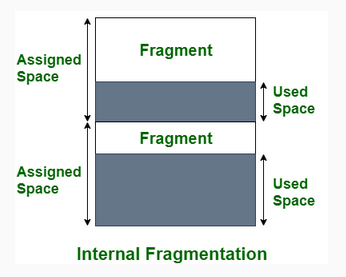
\includegraphics[width=0.55\textwidth]{assets/frag_interna.png}
    \end{center}
\end{figure}

\begin{itemize}
    \item \textbf{Fragmentacion Externa}
        \begin{itemize}
            \item Se produce en el esquema de particiones dinamicas.
            \item Son huecos que van quedando en la memoria a medida que los procesos finalizan.
            \item Puede darse el caso de que tengamos memoria libre para alocar un proceso, pero que no la podamos utilizar.

            \item Una solucion es la \textbf{compactacion}, pero es muy costosa de implementar.
    \begin{figure}
        \begin{center}
            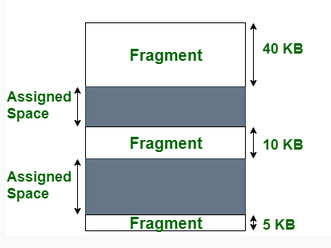
\includegraphics[width=0.55\textwidth]{assets/frag_externa.png}
        \end{center}
    \end{figure}
\end{itemize}
\end{itemize}

\section{Paginacion}
\begin{itemize}
    \item La memoria se divide en porciones de igual tamaño llamadas \textbf{marcos(frames)}.
    \item El espacio de direcciones de los procesos se divide en porciones de igual tamaño llamadas \textbf{paginas)}.
    \item Tamaño de pagina = Tamaño de marco (generalmente 512 bytes).
    \item El SO mantiene una tabla de paginas para cada proceso, que indica en que marco se encuentra cada pagina.
\end{itemize}
\subsection{Direccionamiento}
\begin{itemize}
    \item Un proceso en ejecucion hace referencia a una direccion virtual $v=(p,d)$.
    \item El SO busca la pagina p en la tabla de paginas del proceso y determina en que marco se encuentra.
    \item La direccion de almacenamiento real es formada por la concatenacion de la direccion del marco de p y d, donde d es el desplazamiento.
    \item En este esquema se puede producir fragmentacion interna.
\end{itemize}

\section{Segmentacion}
\begin{itemize}
    \item Se puede ver como un una mejora de la paginacion, en la que no hay fragmentacion interna, sino externa.
    \item Ahora la tabla de segmentos, ademas de tener la direccion del inicio del mismo, tiene la longitud o limite.
    \item Las direcciones logicas constan de un numero de segmento S y un desplazamiento D dentro del segmento.
    \item Todos los segmentos de un programa pueden no tener el mismo tamaño.
    \item El programa es dividido en partes/secciones, donde en cada seccion se guardan datos similares.
\end{itemize}
\subsection{Similitudes/diferencias con las particiones dinamicas}
\begin{itemize}
    \item \textbf{Similitudes:}
\begin{itemize}
    \item Ambas pueden generar fragmentacion externa.
    \item Ambas se basan en la idea de distribuir espacios de tamaño variable a los procesos
\end{itemize}
\item \textbf{Diferencias:}
    \begin{itemize}
        \item El particionamiento dinamico requiere que todo el proceso se encuentre cargado de forma continua en memoria.
        \item La segmentacion subdivide y distribuye las dividiones de forma indiferente a su orden real, aunque si mantiene la secuencia dentro de cada segmento.
    \end{itemize}
\end{itemize}
\subsection{Similitudes/diferencias con la paginacion}
\begin{itemize}
    \item \textbf{Similitudes:}
\begin{itemize}
    \item Ambas tecnicas permiten la distribucion en sectores no contiguos de la memoria.
    \item Se requiere de estructuras adicionales.
\end{itemize}
\item \textbf{Diferencias:}
    \begin{itemize}
        \item La paginacion es transparente al programador, mientras que la segmentacion no.
        \item La paginacion elimina la fragmentacion externa.
        \item La segmentacion facilita modularidad, estructuras de datos grandes y da mejor soporte a la comparticion y proteccion.
    \end{itemize}
\end{itemize}

\section{Memoria Virtual}
\begin{itemize}
    \item Permite ejecutar procesos que requieren mas memoria que la disponible en el sistema.
    \item Mantiene en memoria principal solo aquella memoria que el procesos este utilizando y el resto en disco.
    \item El usuario no debe preocuparse por las limitaciones de la memoria fisica.
    \item El SO debe apoyarse en el hardware, ya que deber ser capaz de detectar cuando se trata de acceder a una direccion que no se encuentra cargada en memoria, y el SO alli podria actuar para atender el fallo.
        \item Para implementar esta tecnica con paginacion por demanda, se requiere como minimo un bit que indique la presencia de la pagina en memoria.
            \item Por otro lado, tambien debe contarse con informacion sobre la presencia de modificaciones en las paginas cargadas, ya que si se descarga una pagina modificada, los datos cargados en el disco deben actualizarse.
\end{itemize}

\subsection{Fallos de pagina (Page Faults)}
\begin{itemize}
    \item Se producen cuando una instruccion ejecutada hace referencia a una direccion logica cuya pagina no se encuentra cargada en memoria pricipal.
    \item El Hardware de la maquina es el responsable de detectar un Page Fault, generando una excepcion para que el sistema operativo se encarge de cargar la pagina en memoria principal.
        \item Acciones del SO al producirse un fallo de pagina:
        \begin{enumerate}
            \item Se genera el trap.
            \item El SO bloquea al proceso actual (la CPU toma otro proceso).
            \item El SO busca un marco libre en la memoria y genera una operacion de E/S que le pide al disco, para copiar en dicho marco la pagina deseada.
            \item La E/s avisa por interrupcion cuando finaliza.
            \item El SO actualiza la tabla de paginas del proceso.
            \item El proceso pasa del estado bloqueado a listo para ejecutar.
        \end{enumerate}
\end{itemize}

\subsection{Tamaño de pagina}
\begin{itemize}
    \item \textbf{Tamaño de pagina pequeño:}
        \begin{itemize}
            \item Menor fragmentacion interna.
    \item Mas paginas requeridas por proceso, por lo que se necesita una tabla de paginas mas grande.
    \item Mas paginas pueden residir en memoria.
\end{itemize}
    \item \textbf{Tamaño de pagina grande:}
        \begin{itemize}
    \item Mayor fragmentacion interna.
    \item Mayor eficiencia al mover paginas hacia la memoria principal.
        \end{itemize}
\end{itemize}

\subsection{Asignacion de marcos}
La asignacion de marco se pueder realizar de dos modos:
\begin{itemize}
    \item \textbf{Asignacion fija:} a cada proceso se le asigna una cantidad arbitraria de marcos. A su vez para el reparto se puede usar:
        \begin{itemize}
            \item \textbf{Reparto equitativo:} se asigna la misma cantidad de marcos a cada proceso : $m / p$
            \item \textbf{Reparto proporcional:} se asignan marcos en base a la necesidad de cada proceso : $V_p \cdot m /V_t$
                \begin{itemize}
                    \item $m$: cantidad de marcos.
                    \item $V_p$: paginas usadas por el proceso.
                    \item $V_t$: paginas usadas en total por todos los procesos.
                \end{itemize}
        \end{itemize}
        \item \textbf{Asignacion dinamica:} se asignan marcos a los procesos segun la demanda.
\end{itemize}


\section{Reemplazo de paginas}
\begin{itemize}
    \item Cuando se produce un fallo de pagina, el SO debe decidir que pagina reemplazar.
    \item El objetivo es minimizar el numero de fallos de pagina.
    \item \textbf{Algoritmos de reemplazo de paginas:}
        \begin{itemize}
            \item \textbf{FIFO:} Se reemplaza la pagina que esta en memoria hace mas tiempo.
            \item \textbf{LRU:} Se reemplaza la pagina que no se ha utilizado hace mas tiempo. Favorece a las paginas menos recientemente accedidas.
            \item \textbf{FIFO (Segunda Chance:)} 
                \begin{itemize}
                    \item Se utiliza un bit adicional, llamado bit de referencia.
                    \item Cuando la pagina se carga en memoria, el bit R se pone en 0.
                    \item Cuando la pagina es referenciada, el bit R se pone en 1.
                    \item La victima se busca en orden FIFO. Se selecciona la primer pagina cuyo bit R esta en 0.
                    \item Mientras se busca a la victima, cada bit R que tiene el valor 1, se cambia a 0.
                \end{itemize}
        \end{itemize}
        \item Cuando una pagina que fue modificada es reemplazada, se reserva uno o varios marcos para la descarga asincronica de paginas.
            \begin{enumerate}
                \item La pagina que provoco el fallo se coloca en un frame designado a la descarga asincronica.
                \item El SO envia la orden de descargar asincronicamente la pagina modificada mientras continua la ejecucion de otro proceso.
                \item El frame de descarga asincronica pasa a ser el que contiene la pagina victima que ya se descargo correctamente.
            \end{enumerate}
\end{itemize}
\subsection{Alcance del reemplazo}
\begin{itemize}
    \item \textbf{Reemplazo local}
        \begin{itemize}
            \item El fallo de pagina de un proceso solo puede reemplazar sus propias paginas.
            \item No cambia la cantidad de frames asignados.
            \item El SO puede determinar cual es la tasa de page-faults de cada proceso.
            \item Un proceso puede tener frames asignados que no usa, y no pueden ser usador por otros procesos.
        \end{itemize}
        \item \textbf{Reemplazo global}
            \begin{itemize}
                \item El fallo de pagina de un proceso puede reemplazar la pagina de cualquier proceso.
                \item El SO no controla la tasa de page-faults de cada proceso.
                \item Puede tomar frames de otro proceso, aumentando la cantidad de frames asignados a el.
                \item Un proceso de alta prioridad podria tomar los frames de un proceso de menor prioridad.
            \end{itemize}
\end{itemize}


\section{Hiperpaginacion (Trashing)}
\begin{itemize}
    \item Un sistema esta en estado de hiperpaginacion cuando pasa mas tiempo paginando que ejecutando procesos.
    \item Generalmente sucede cuando el total de marcos disponibles en el sistema es inferior a la suima de los conjuntos de trabajo de cada proceso en ejecucion. Es decir, cuando los procesos en ejecucion no tienen suficientes marcos asignados como para mantener su conjunto de trabajo.
    \item El SO, puede detectarlas mediante el control de la frecuencia de fallos de pagina.
    \item Se pueden reasignar marcos de un proceso a otro.
\end{itemize}
\subsection{Anomalia de Belady}
\begin{itemize}
    \item Ocurre cuando al aumentar el numero de marcos en la memoria fisica, usando el algoritmo FIFO, aumenta el numero de Page-Faults.
\end{itemize}
\end{document}
